\section{Introduction}
\label{sec:intro}

Large language models (LLMs) are increasingly deployed as
knowledge-intensive components of production software systems, powering
question answering over enterprise documents, regulatory and financial
assistants, and clinical decision support
\citep{lewis2020rag,gao2023alce,yang2024cragbench,aarab2025bank,
yang2025integrating}. Because parametric
knowledge is incomplete, stale, and prone to hallucination,
retrieval-augmented generation (RAG) has become the default mechanism
for grounding LLM outputs in external knowledge sources --- relational
tables, text corpora under sparse and dense indexes, vector stores, and
structured knowledge APIs \citep{lewis2020rag,chen2020hybridqa}. A
modern RAG service is therefore a \emph{knowledge acquisition pipeline}:
between retrieval and generation sit fusion, reranking, verification,
and a menu of LLMs whose per-token prices span two orders of magnitude.
The same information need admits many pipeline configurations, and
their cost differences are large; their quality differences are real
but stochastic. For knowledge services that face compliance, safety, or
service-level obligations, a property more fundamental than average
accuracy is at stake: \emph{can the operator state, before violations
reach users, what fraction of answers will fail the application's
quality, citation, freshness, or latency requirements?}

\begin{figure*}[t]
\centering
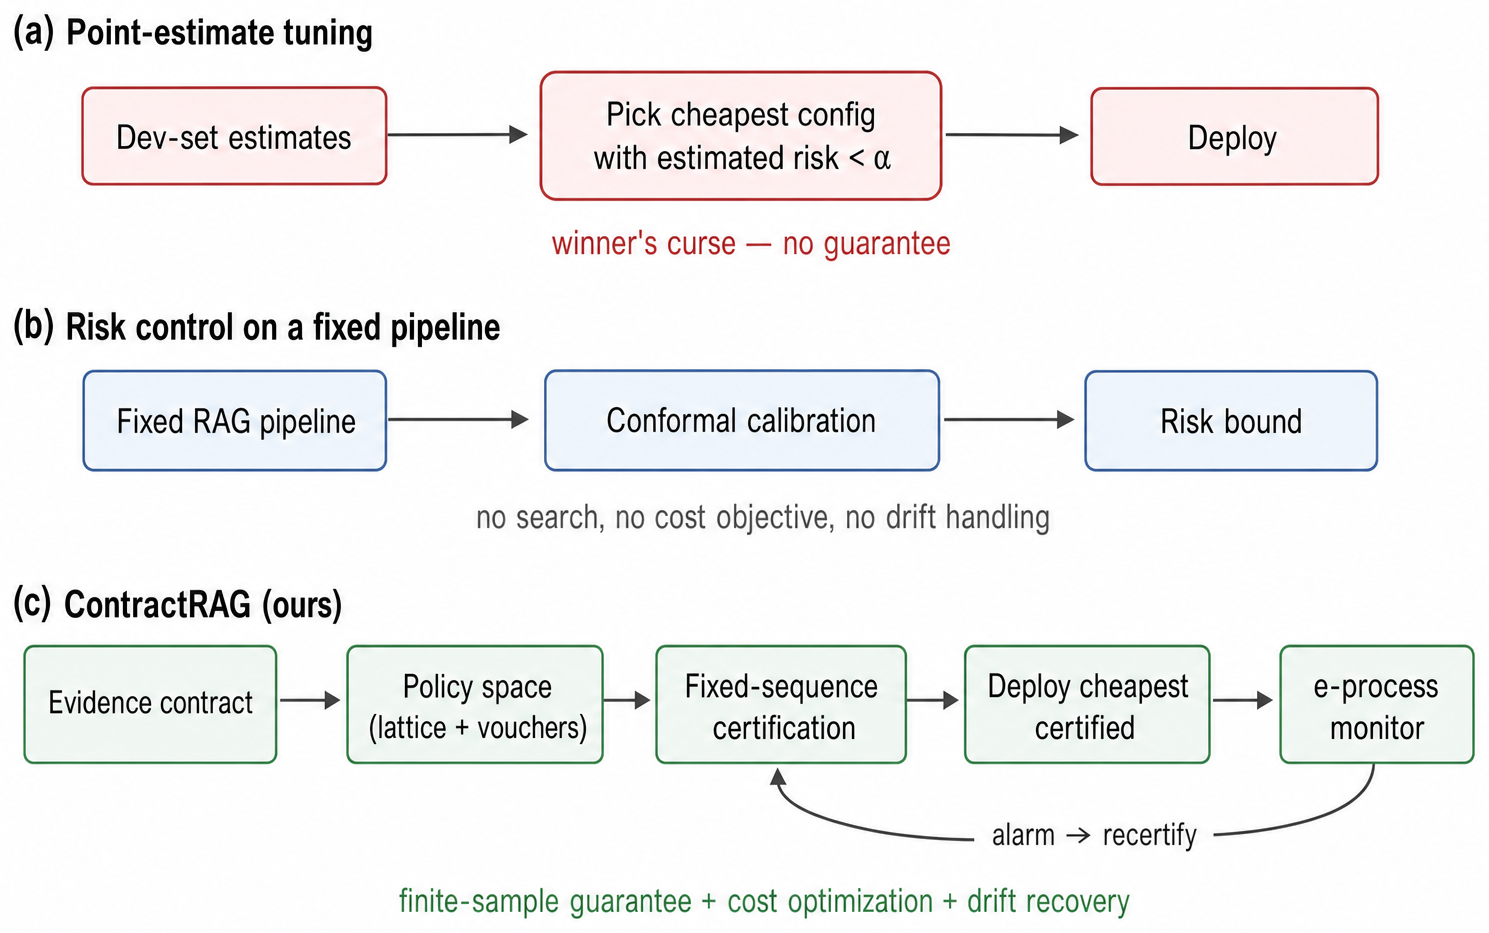
\includegraphics[width=0.88\textwidth]{figures/fig_paradigm.png}
\caption{Three deployment paradigms for RAG knowledge services.
(a)~Point-estimate tuning deploys the cheapest configuration whose
\emph{measured} risk clears the target --- an uncorrected
multiple-testing procedure with no feasibility guarantee.
(b)~Distribution-free risk control bounds the risk of a \emph{fixed}
pipeline but neither searches a configuration space nor reduces cost,
and is silent under drift. (c)~\system\ unifies search, certification,
and monitoring: an evidence contract is certified by a fixed-sequence
test over a policy space ordered by risk vouchers, and an anytime-valid
e-process monitor closes the loop after deployment.}
\label{fig:paradigm}
\end{figure*}

However, the dominant deployment practice cannot answer this question.
Practitioners sample a development set, estimate each configuration's
quality, and deploy the cheapest configuration whose \emph{estimate}
clears the target --- a paradigm we call point-estimate tuning
(Figure~\ref{fig:paradigm}a), shared
by workload-level pipeline optimizers \citep{russo2025abacus,
liu2025palimpzest,patel2024lotus} and by adaptive RAG routers and LLM
cascades \citep{jeong2024adaptiverag,chen2023frugalgpt,ong2024routellm}.
This paradigm suffers from a fundamental statistical flaw: selecting
the cheapest configuration whose measured risk clears a threshold is a
multiple-testing procedure without a correction, so the winner is
systematically the configuration whose noise broke in its favor. The
failure is structural rather than a matter of tuning budget --- more
candidates make it worse, not better. As we quantify in
Section~\ref{sec:results}, state-of-practice optimizers deploy policies
whose true violation rate exceeds the declared target in up to 64\% of
calibration draws: for a compliance requirement, a coin flip. Moreover,
even a correctly tuned pipeline offers no protection after deployment,
when workload mix shifts, indexes fall behind the world, and knowledge
APIs degrade --- the knowledge drift problem that static evaluation
cannot see.

Distribution-free risk control offers a principled remedy
(Figure~\ref{fig:paradigm}b): conformal
and Learn-then-Test methods \citep{angelopoulos2021ltt,
angelopoulos2024crc} can bound the violation rate of a \emph{fixed}
pipeline with finite-sample confidence, and recent work has applied
them to RAG abstention and answer sets \citep{li2024traq,kang2024crag}.
Yet these methods treat the pipeline as given: they neither search a
configuration space nor reduce cost, and they are silent about what
happens when the calibrated distribution drifts. Conversely, the
systems that do search --- routers, cascades, Bayesian optimization ---
provide no feasibility statement at all. What is missing is a framework
in which \emph{search, certification, and post-deployment monitoring}
are designed together, so that cost optimization never erodes the
statistical guarantee.

To close this gap, we propose \system, a certified deployment framework
for RAG knowledge services (Figure~\ref{fig:paradigm}c). The key idea
is to make the reliability
promise a first-class, declarative object: an \emph{evidence contract}
states admissible violation rates for answer quality, citation
completeness, evidence freshness, and latency, together with a
confidence budget $\delta$ for the certification itself. \system\ then
treats contract feasibility the way a database treats integrity
constraints: no pipeline configuration --- however attractive its point
estimate --- is deployable unless a statistical test on calibration
executions certifies it. Three mechanisms make this practical. First,
cost-decreasing pipeline rewrites (retrieval truncation, reranker
elision, pre-filter pushdown, generator downgrade) are annotated with
empirical \emph{risk vouchers} --- confidence upper bounds on their
probability of harming an answer --- which compose assumption-free
along rewrite chains by a telescoping argument and guide the search the
way a cost model guides a query optimizer: they order candidates but
never justify the deployment. Second, the rewrite lattice is lifted
into \emph{progressive knowledge-acquisition policies} --- escalation
ladders that execute cheap plans first and escalate while runtime
sufficiency evidence is inadequate, cost-utility routers, and
group-conditional variants, and, under strict contracts, policies that
defer residual queries to human review with a certified deferral
budget --- and a fixed-sequence Hoeffding--Bentkus test certifies a
feasible low-cost policy (the cheapest of its certified prefix) with
no multiplicity penalty, so enriching the policy space never erodes
the guarantee. Third, an anytime-valid restart-mixture e-detector
watches deployed violations --- at full or subsampled audit rates ---
with a change-time-independent detection-delay bound, localizes the
changepoint at $O(1)$ cost per query, and drives a closed-loop
certified recalibration procedure whose geometric error-budget
schedule remains valid over arbitrarily many alarms. This design elevates RAG
deployment from point-estimate tuning to certified knowledge-service
management: learned components decide how much money the certified
policy saves, while statistics alone decides whether the contract
holds.

To the best of our knowledge, this is among the first frameworks to
provide end-to-end, finite-sample reliability guarantees for
cost-optimized RAG over heterogeneous knowledge sources. The main
contributions of this paper are summarized as follows:
\begin{itemize}
\item We propose \emph{evidence contracts}, a declarative and
statistically meaningful interface between knowledge-intensive
applications and the RAG execution layer, subsuming quality, citation,
freshness, and latency requirements
(Section~\ref{sec:prelim}).
\item We design a certified plan optimizer that combines
rewrite-generated plan lattices, assumption-free telescoping voucher
composition, selectivity-conditioned vouchers, and
cardinality-driven knowledge-source selection, with fixed-sequence
testing as the sole source of soundness; we prove contract validity for
any candidate count and any score quality, and a cost-consistency
guarantee (Section~\ref{sec:method}).
\item We develop an anytime-valid drift monitor based on a
restart-mixture e-detector, with a proven change-time-independent
detection delay bound, $O(1)$ changepoint localization, validity under
subsampled auditing, a certified post-alarm recalibration loop, and a
lifetime guarantee across repeated alarms via geometric error spending
(Section~\ref{sec:monitor}).
\item We conduct a systematic empirical study on four heterogeneous
benchmarks with fully metered execution across four LLM families from
four model developers on two serving backends (token- and
GPU-second-metered). Verified directly on exact finite-population
risk, \system\ is the only method meeting its contract budget
everywhere (violation probability at most 0.8\% over 1000 draws
against $\delta=10\%$); it cuts cost by up to 20$\times$ against the
strongest fixed pipeline (10--18$\times$ after charging monitoring
audits), certifies strict contracts down to $\alpha = 0.1$ with
deferral and four-constraint joint contracts where Bonferroni
certifies nothing, detects injected drift in a median of 78 queries
with no false alarms, and reports infeasibility honestly when no
configuration can meet the contract
(Sections~\ref{sec:setup}--\ref{sec:results}).
\end{itemize}

The remainder of this paper is organized as follows.
Section~\ref{sec:related} reviews related work.
Section~\ref{sec:prelim} formalizes evidence contracts and the
certified deployment problem. Section~\ref{sec:method} presents the
\system\ framework. Sections~\ref{sec:setup} and~\ref{sec:results}
report the experimental setup and results. Section~\ref{sec:discussion}
discusses implications, limitations, and threats to validity, and
Section~\ref{sec:conclusion} concludes.
